\begin{frame}{A single edge}
\begin{columns}[T,onlytextwidth]
	\begin{column}{0.5\textwidth}
        \vspace{.5em}
		\centering
        \begin{tikzpicture}[scale=3.5]
            \node[circle, fill, inner sep=1.5pt, label=left:\(v\)] (v) at (0,0) {};
            \node[circle, fill, inner sep=1.5pt, label=left:\(w\)] (w) at (0,1) {};
            \draw (v) -- (w);
        \end{tikzpicture}
        
        \vspace{1em}
		\scriptsize \(\Gamma\) is a single edge
	\end{column}

	\begin{column}{0.5\textwidth}
		\centering
        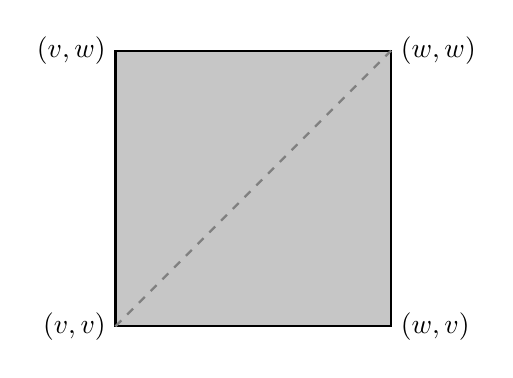
\begin{tikzpicture}[scale=3.5]
            \fill[gray, opacity=0.45] (0,0) rectangle (1,1);
            \draw[thick] (0,0) rectangle (1,1);
            \node[left] (vv) at (0,0) {\((v, v)\)};
            \draw[gray, dashed, thick] (0,0) -- (1,1);
            \node[right] (ww) at (1,1) {\((w, w)\)};

            \node[left] (ww) at (0,1) {\((v, w)\)};
            \node[right] (ww) at (1,0) {\((w, v)\)};
        \end{tikzpicture}

        \vspace{1em}
		\scriptsize \(\Conf_2(\Gamma)\)
    \end{column}
\end{columns}
\end{frame}